\chapter{Internet Trends}

\section{Web zum Ersten}

Das Web 1.0 war der \textbf{erste konzeptionelle Entwicklungsschritt} des Internet. Es war eine Sammlung von Websites mit dem Ziel der Publikation und Präsentation von Informationen. Die Informationen können aufgerufen aber nicht verändert werden (man befürchtete Datensicherheitsrisiken). Es gab viele Nutzer und wenig Anbieter (Firmen, persönliche Websites) von Inhalten. Es handelte sich meist um statische HTML-Seiten, welche ein GIF oder ein Guestbook anbieteten um mit dem Benutzer zu interagieren. Nachfolgend ein kurzer Überblick über die Geschichte des Internets:
\begin{description}
	\item[1969] Erste ARPANET Übertragung
	\item[1980] Ethernet Standard wird eingeführt
	\item[1982] TCP/IP Protokoll definiert
	\item[1986] Internet Engineering Task Force (IETF)
	\item[1991] World Wide Web (www) von Tim Berners-Lee
	\item[1993] www öffentlich zugängig
	\item[1995] IPv6 vorgestellt (WTF?)
	\item[1995] Amazon.com, eBay	(Online Shopping)
	\item[1996] Hotmail
	\item[1998] Google Search, Yahoo!, PayPal
	\item[1999] Napster (Filesharing)
	\item[2000] dot-com bubble
	\item[2001] BitTorrent, Wikipedia
	\item[2003] LinkedIn, MySpace, iTunes, Skype	(Social Media)
	\item[2004] Facebook, Flickr
	\item[2005] YouTube
	\item[2006] Twitter
	\item[2008] Amazon Elastic Compute Cloud (EC2), Dropbox (Cloud Dienste)
	\item[2009] Google Docs (Web-basierende Textverarbeitung)
	\item[2009] Bitcoin
	\item[2010] Instagramm (Social networking und Photo sharing)
	\item[2011] Google+ (Social networking und identity Dienste)
\end{description}

\section{Web 2.0}

Das Web 2.0 war der \textbf{zweite konzeptionelle Entwicklungsschritt} des Internet. Web 1.0 wurde erst nachträglich so benannt. Unterstützt durch neue Technologien, veränderte sich die Nutzung des Internets (ca. ab 2004). Die Websites werden \textbf{interaktiv}. Die Inhalte werden durch die Nutzer definiert, mit dem Ziel einer dynamischen Sammlung und Verwaltung von Informationen. Die Rollen von Anbietern und Nutzern verschwimmen da jeder zum Bearbeiter (Prosumer) wird. Im Web gibt es keinen klassischen Software Lebenszyklus mehr. Die Inhalte sind immer im Beta-Stadium und verändern sich in neue und nie beabsichtigte Formen. Dieser Fluss kann auch ausser Kontrolle geraten (shitstorm, cyber mobbing). Zudem sind die Inhalte hoch-dynamisch crowd-basiert (kollektive Intelligenz). Es ist ein Übergang von Push (aktive Verteilung) zu Pull (aktive Sammlung).

\section{Semantic Web}

Zurzeit besteht das Web aus einer Sammlung von verlinkten HTML-Dokumenten. Die Struktur der Informationen ist \textbf{generisch} (nicht strukturiert) und die Bedeutung der Inhalte lässt sich nur aus dem Kontext schliessen (\textbf{implizit}). Die Inhalte sollen vor allem \textbf{für Menschen} lesbar sein.

Beim Semantic Web (oder auch Web 3.0) soll das Internet \textit{intelligent} werden. Maschinen sollen die Bedeutung von Informationen verstehen und können diese basierend auf deren Bedeutung verarbeiten. Um dies zu erreichen ist der primäre Inhalt nicht mehr ein HTML-Dokument sondern eine \textit{Sache}. Diese Sachen stehen in Beziehung zueinander. Die Struktur der Information, wird basierend auf einem RDF Datenmodell, \textbf{generell definiert}. Die Bedeutungen der Inhalte und der Vernetzungen sind \textbf{explizit}. Dadurch werden die Inhalte für \textbf{Mensch und Maschinen} lesbar.

Eine semantische Information könnte folgende Aussage sein:
\begin{quote}
	\textit{«Billet für das Rolling Stones Konzert im KKL im Januar»}
\end{quote}
Ein Mensch versteht implizit dass ein Billet für ein Rolling Stones Konzert gesucht wird. Ausserdem weiss man dass \textit{Billett} die gleiche Bedeutung wie Ticket, Karte oder Eintrittskarte hat. Man nimmt auch an dass \textit{KKL} ein Ort für Anlässe und \textit{Januar} ein Datum ist. Im Semantic Web können solche semantische Zusammenhänge \textit{maschinenlesbar} erfasst werden.

Um dieses Ziel zu erreichen muss man die Bedeutung von Informationen verstehen und interpretieren. Dazu müssen bestehende Informationen mit Metadaten annotiert werden. Die Struktur einer Information kann mit der auf XML basierenden Beschreibungssprache RDF (Resource Description Framework) beschrieben werden. Um Informationen über logische Beziehungen (z.B. Hierarchie) zu beschreiben kann die OWL (Web Ontology Language) verwendet werden.

Nachdem die Bedeutung der Informationen verstanden wurde, kann man es für neue Schlussfolgerungen interpretieren. Dazu kann man Abfrage z.B. mit SPARQL (SPARQL Protocol And RDF Query Language) durchführen oder Regeln mit z.B. RIF (Rule Interchange Format) formulieren. Es gibt auch Tools wie Protégé, um QWL-basierende Wissensdatenbanken anzulegen und abzufragen. Abbildung \ref{fig:semantic-webstack} zeigt den Technologiestack des Semantic Web.
\begin{figure}
\centering
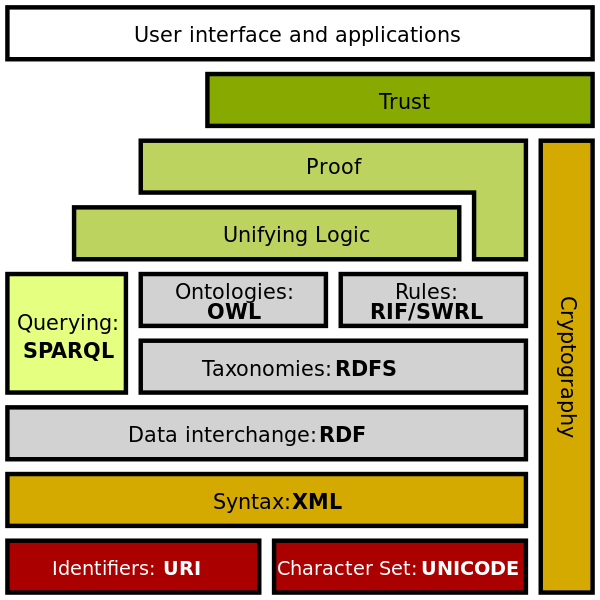
\includegraphics[width=0.5\linewidth]{fig/semantic-webstack}
\caption{Stack des Semantic Web}
\label{fig:semantic-webstack}
\end{figure}
Möchte man solche Systeme bauen, wird man mit diesen Herausforderungen konfrontiert:
\begin{description}
	\item[Vastness] Die Datenmenge ist riesig (4.74 Milliarden Websites im Oktober 2014)
	\item[Vagueness] Teilweise ist unklar was eine Benutzeranfrage genau meint (Ab wann ist man \textit{alt}?).
	\item[Uncertainty:] Präzise Konzepte mit unsicheren Werten (Was auch immer das heisst).
	\item[Inconsistency] Inkonsistente Informationen (z.B. Auto hat Sitze, Motor, Zylinder vs. Auto hat Sitze und Motor, Motor hat Zylinder).
	\item[Deceit] Der Anbieter von Informationen kann den Benutzer betrügen (z.B. Das günstigste Auto).
\end{description}
Im Semantic Web gibt es einige Begriffe die nachfolgend definiert werden:
\begin{description}
	\item[Ontologien (Taxonomien):] in der Informatik sind meist sprachlich gefasste und formal geordnete Darstellungen einer Menge von Begrifflichkeiten und der zwischen ihnen bestehenden Beziehungen in einem bestimmten Gegenstandsbereich z.B. ein Ordnungssystem von Tieren oder von Pflanzen, oder von öffentlichen Verkehrsmitteln.
	\item[Inference-Engine (Reasoner)] Software, die anhand von bekannten Zusammenhängen, neue \textit{folgert} oder \textit{ableitet}. Diese neuen Zusammenhänge sind \textit{bewiesen}. Als Beispiel wenn ich in meinem Büro bin und mindestens eine andere Person anwesend ist und meine Türe geschlossen ist, dann bin ich in einer Sitzung. Wenn ich in einer Sitzung bin dann möchte ich nicht gestört werden und mein Telefon soll automatisch auf Voicemail umgeleitet werden.
\end{description}

\subsection{Resource Description Framework (RDF)}

Mit RDF lassen sich Informationen im Web repräsentieren. Ein RDF-Statement besteht immer aus einer Ressource die eine Beziehung (Property) zu einer anderen Ressource hat. Dies wird auch triple-store genannt. Eine Ressource ist eine Sache (ein Ding) (virtuell oder real), das eine URI (Uniform Resource Identifier) hat, oder ein Literal (konstanter Wert) ist. Eine Property ist eine spezielle Art von Ressource, die dazu dient, eine gerichtete Beziehung zwischen zwei anderen Ressourcen herzustellen. Listing \ref{lst:rdf} zeigt ein Beispiel für eine RDF-Datei. \verb|rdf:RDF| ist das Root-Element einer RDF-Datei und spezifiziert zwei Namespaces (\verb|rdf| und \verb|cd|). \verb|rdf:Description| definiert eine Ressource welche über das \verb|rdf:about|-Attribut identifiziert wird. Die Elemente \verb|cd:artist|, \verb|cd:country| usw. sind Properties der Ressource, welche ein Literal als Wert haben.

\begin{lstlisting}[language=XML, caption=RDF Beispiel, label=lst:rdf]
<?xml version="1.0"?>

<rdf:RDF
xmlns:rdf="http://www.w3.org/1999/02/22-rdf-syntax-ns#"
xmlns:cd="http://www.recshop.fake/cd#">

<rdf:Description rdf:about="http://www.recshop.fake/cd/Empire Burlesque">
	<cd:artist>Bob Dylan</cd:artist>
	<cd:country>USA</cd:country>
	<cd:company>Columbia</cd:company>
	<cd:price>10.90</cd:price>
	<cd:year>1985</cd:year>
</rdf:Description>

</rdf:RDF>
\end{lstlisting}

\subsection{Web Ontology Language (OWL)}

OWL ist eine Erweiterung von RDF welche zusätzliche Ressourcen einführt, dessen Bedeutung gut definiert ist. Basiert ebenfalls auf XML und kann graphisch dargestellt werden (z.B. Protégé). Listing \ref{lst:owl} beschreibt die Begriffe \verb|<Person>|, \verb|<Gender>| und \verb|<Woman>|. Eine Frau ist definiert als eine <Person> mit dem Wert \verb|<female>| im Property \verb|<gender>|, das der Klasse \verb|<Gender>| angehören muss. Die Instanz \verb|<STilgner>| ist somit als \verb|<Person>| beschrieben eine Frau (\verb|<Woman>|). 

\begin{lstlisting}[language=XML, caption= OWL Beispiel, label=lst:owl]
<rdf:RDF
	xmlns:rdf="http://www.w3.org/1999/02/22-rdf-syntax-ns#"
	xmlns:rdfs="http://www.w3.org/2000/01/rdf-schema#"
	xmlns:owl="http://www.w3.org/2002/07/owl#"
	xmlns="http://localhost:8080/OWLBuergerInformation.owl#"
	xml:base="http://localhost:8080/OWLBuergerInformation.owl">

	<owl:Ontology rdf:about=""/>   
	
	<owl:Class rdf:ID="Gender"/>
	<owl:Class rdf:ID="Person"/> 
	<owl:Class rdf:ID="Woman">
		<rdfs:subClassOf rdf:resource="#Person"/>
		<owl:equivalentClass>
			<owl:Restriction>
				<owl:onProperty rdf:resource="#gender"/>
				<owl:hasValue rdf:resource="#female" rdf:type="#Gender"/>
			</owl:Restriction>
		</owl:equivalentClass>
	</owl:Class>
	
	<owl:ObjectProperty rdf:ID="gender"
	rdf:type="http://www.w3.org/2002/07/owl#FunctionalProperty">
		<rdfs:range rdf:resource="#Gender"/>
		<rdfs:domain rdf:resource="#Person"/>
	</owl:ObjectProperty>
	<owl:DatatypeProperty rdf:ID="name"
	rdf:type="http://www.w3.org/2002/07/owl#FunctionalProperty">
		<rdfs:range rdf:resource="http://www.w3.org/2001/XMLSchema#string"/>
		<rdfs:domain rdf:resource="#Person"/>
	</owl:DatatypeProperty>
	<owl:DatatypeProperty rdf:ID="firstname"
	rdf:type="http://www.w3.org/2002/07/owl#FunctionalProperty">
		<rdfs:range rdf:resource="http://www.w3.org/2001/XMLSchema#string"/>
		<rdfs:domain rdf:resource="#Person"/>
	</owl:DatatypeProperty>
	
	<Person rdf:ID="STilgner" firstname="Susanne" name="Tilgner">
		<Gender rdf:resource="#female"/>
	</Person>
</rdf:RDF>
\end{lstlisting}

\section{Internet of Things (IoT)}

Mark Weiser (Chief Scientist at Xerox PARC) hat die Vision des Ubiquitous Computing als Computer Model für das 21. Jahrhundert vorgestellt. Ubiquitous bedeutet so viel wie Allgegenwärtig und im Hintergrund. Dabei soll die richtige Information, am richtigen Ort und zur richtigen Zeit den Benutzer erreichen. Im IoT werden physikalische Dinge ans Internet angeschlossen. Dinge haben Sensoren und Aktoren mit denen die reale Welt gemessen und beeinflusst wird. Dieses Abbild (Modell) der realen Welt kann so in die virtuelle Welt übertragen werden (Sensoren) bzw. die virtuelle Welt kann so die reale Welt beeinflussen (Aktoren). Um das IoT zu realisieren braucht es:
\begin{description}
	\item[Intelligente Dinge] Dinge mit Sensoren, Aktoren, Rechenleistung und mit einer Netzwerkverbindung
	\item[Netzwerke] Technologien um die einzelnen Netzwerke (Dinge) und deren Informationen zu verbinden und zu integrieren
	\item[Intelligente Applikationen] Informationen werden gesammelt, verarbeitet und interpretiert. Intelligente Entscheidungen werden in entsprechende Aktionen/Aktivitäten umgesetzt
\end{description}
Zurzeit ist leider nur 1\% der Dinge um uns herum mit dem Internet verbunden. Kühlschrank, Auto, Waschmaschine usw. sollten verbunden werden, sind es aber nicht (OMG! Wa machemr jetzt?!). Aber das IoT wird das nächste grosse Ding weil es bei Gartner auf Platz 3 steht. Zurzeit wird das IoT in folgenden Gebieten eingesetzt:
\begin{itemize}
	\item Gebäudeautomation (Smart TV, Stereo, Storen, Heizung, Klimaanlage, Alarmanlage)
	\item Smart Grid (dynamische Energieverteilung, Optimierung des Verbrauchs, Fehlersuche)
	\item Verkehr (Verkehrsamplen, Real-time Informationssysteme)
	\item Automotive (Smart Cars, Ferndiagnose, In-Car)
	\item Industrie (Automatisierte Abläufe, Assembly Lines, Lager, RFID)
	\item Healthcare (Unterstützung im Alter, Ferndiagnosen, Fernoperationen)
\end{itemize}
Im IoT haben sich diese Interaktionspattern herausgebildet:
\begin{description}
	\item[M2M (Machine to Machine)] Dinge arbeiten zusammen (kollaborieren) um das tägliche Leben automatisch und im Hintergrund zu unterstützen
	\item[M2P (Machine to Person)] Anwender (und/oder Server) benutzen Dinge zur Informationsabfrage, Fernbedienung, Fernsteuerung
	\item[M2C (Machine to Cloud)] Dinge sammeln Informationen und speichern diese in der Cloud. Irgendjemand wird diese Informationen dann irgendwann auswerten/benutzen.
\end{description}
Zudem müssen noch folgende Aspekte beachtet werden:
\begin{itemize}
	\item Datensicherheit
	\item Personensicherheit
	\item Zugriffsberechtigungen
	\item \textbf{big borther}
	\item Datenschutz
	\item National, international
\end{itemize}

Die Dinge verschwinden in den Hintergrund und sie verhalten sich wie Objekte in OOP. Sie sind miteinander vernetzt und interagieren miteinander.

\section{Internet of Everything (IoE)}

Das IoE ist möglicherweise der nächste Evolutionsschritt des Internets. Es ist ein Netzwerk von Netzwerken (also ist es heute schon oder nicht?), in dem IoT, Menschen, Daten und Prozesse integriert sind. Die richtigen Informationen, am richtigen Ort, zur richtigen Zeit, mit der richtigen Qualität!

\textit{So und jetzt weiss ich nicht was ich über diesen Gspass noch schreiben soll\dots}